\documentclass[aspectratio=169,dvipsnames,svgnames,10pt]{beamer}

\usepackage[T1]{fontenc}
\usepackage[utf8]{inputenc}
\usepackage[french, english]{babel}
\selectlanguage{english}

\usepackage{graphicx}

% Math
\usepackage{amsmath}
% \usepackage{amsfonts}
\usepackage{amssymb}
\usepackage{amsthm}
% \usepackage{mathrsfs}
\usepackage{mathtools}
\usepackage{textcomp}
% \usepackage{textgreek}

% Specialized packages
% \usepackage{syntax} % Grammar definitions
\usepackage{verbatim}
\usepackage{listings} % Code
\usepackage{xspace} % Useful for macros
\usepackage{natbib}% Good citations and bibliography
\usepackage{mathpartir} % Syntax trees
\usepackage{colortbl}
\usepackage{hhline}
\usepackage{multicol}%multicolumn lists
\usepackage{pifont}%% check mark
\usepackage{minted}
\usepackage{wasysym}

% \usepackage{mathptmx}
% \usepackage[scaled=0.9]{helvet}
\usepackage{beramono}

\bibliographystyle{ACM-Reference-Format}
\citestyle{acmauthoryear}
\usepackage{appendixnumberbeamer}

\usetheme{metropolis}
\beamertemplatenavigationsymbolsempty
\setbeamercovered{transparent=20}
\metroset{
  sectionpage=none,
  numbering=fraction,
  progressbar=foot,
}

\usepackage{tikz}
\usetikzlibrary{decorations.text,backgrounds,positioning,shapes,
  shadings,shadows,arrows,decorations.markings,calc,fit,fadings,
  tikzmark,scopes
}

\tikzset{
  annot/.style={draw=black,scale=0.9,rounded corners=6pt, thick},
  onslide/.code args={<#1>#2}{\only<#1>{\pgfkeysalso{#2}}},
  overline/.style={
    opacity=.2, inner xsep=2pt, inner ysep=0.5em, yshift=3pt, minimum height=11pt
  },
  code/.style={overline,rounded corners=6pt,fill=Blue},
}
\tikzstyle{link}=[->,>=latex, rounded corners=6pt, thick]
\newcommand\tikzcoord[1]{%
  \tikz[baseline,remember picture]{\node[coordinate] (#1) {};}}


\def\HUGE{\fontsize{35pt}{15pt}\selectfont}

\newcommand\htag[1]{\shortintertext{\textbf{#1}}}

\newcommand\TODO[1]{{\ \\\color{red}\large\textbf{TODO} #1}\\}

%%% Local Variables:
%%% mode: latex
%%% TeX-master: "main"
%%% End:

\usepackage{xcolor}
%\definecolor{butter}{HTML}{FCE94F}
%\definecolor{butter}{HTML}{EDD400}
\definecolor{butter}{HTML}{C4A000}
%\definecolor{orange}{HTML}{FCAF3E}
%\definecolor{orange}{HTML}{F57900}
\definecolor{orange}{HTML}{CE5C00}
%\definecolor{chocolate}{HTML}{E9B96E}
%\definecolor{chocolate}{HTML}{C17D11}
\definecolor{chocolate}{HTML}{8F5902}
%\definecolor{chameleon}{HTML}{8AE234}
%\definecolor{chameleon}{HTML}{73D216}
\definecolor{chameleon}{HTML}{4E9A06}
%\definecolor{skyblue}{HTML}{729FCF}
%\definecolor{skyblue}{HTML}{3465A4}
\definecolor{skyblue}{HTML}{204A87}
%\definecolor{plum}{HTML}{AD7FA8}
%\definecolor{plum}{HTML}{75507B}
\definecolor{plum}{HTML}{5C3566}
%\definecolor{scarletred}{HTML}{EF2929}
%\definecolor{scarletred}{HTML}{CC0000}
\definecolor{scarletred}{HTML}{A40000}
%\definecolor{lightalu}{HTML}{EEEEEC}
%\definecolor{lightalu}{HTML}{D3D7CF}
\definecolor{lightalu}{HTML}{BABDB6}
%\definecolor{darkalu}{HTML}{888A85}
%\definecolor{darkalu}{HTML}{555753}
\definecolor{darkalu}{HTML}{2E3436}

\newcommand{\kwstyle}{}

\lstset{
% backgroundcolor=\color{},
        basicstyle=\scriptsize\ttfamily,
% breakatwhitespace=false,
  breaklines=true,
% captionpos=b,
        aboveskip=5pt,
        belowskip=5pt,
        xleftmargin=0pt,
  commentstyle=\color{orange},
  % columns=[c]spaceflexible,
  % flexiblecolumns=false,
% deletekeywords={...},
% extendedchars=true,
% frame=l,
% keepspaces=true,
  keywordstyle=\kwstyle,
  language=Caml,
% morekeywords={*,...},
% numbers=left,
% numbersep=5pt,
% numberstyle=\color{},
% rulecolor=\color{},
% showspaces=false,
% showstringspaces=false,
% showtabs=false,
% stepnumber=2,
  stringstyle=\color{plum},
  tabsize=2,
  numberstyle=\tiny\color{gray},
  escapeinside={(*@}{*)},
  numbers=left,
  numbersep=2pt,
% title=\lstname,
  keywordstyle=[1]\kwstyle\color{chameleon},
  keywordstyle=[2]\kwstyle\color{scarletred},
  keywordstyle=[3]\kwstyle\color{skyblue},
  keywordstyle=[4]\kwstyle\color{butter},
  keywordstyle=[5]\kwstyle\color{skyblue},
  keywordstyle=[6]\kwstyle\color{skyblue},
  keywordstyle=[7]\kwstyle\color{chameleon},
  keywordstyle=[8]\kwstyle\color{butter},
  keywordstyle=[9]\kwstyle\color{butter},
  keywords=[1]{let,val,method,in,and,rec,private,virtual,constraint},
  keywords=[2]{type,open,class,module,exception,external},
  keywords=[3]{fun,function,functor,match,try,with},
  keywords=[4]{as,when,of},
  keywords=[5]{if,then,else},
  keywords=[6]{begin,end,object,struct,sig,for,while,do,done,to,downto},
  keywords=[7]{true,false},
  keywords=[8]{include,inherit,initializer},
  keywords=[9]{new,ref,mutable,lazy,assert,raise},
  keywords=[10]{lin,aff,un},
}

\lstset{literate=
  % {0}{{{\kwstyle\color{plum}0}}}1 {0.}{{{\kwstyle\color{plum}0.}}}2
  % {1}{{{\kwstyle\color{plum}1}}}1 {1.}{{{\kwstyle\color{plum}1.}}}2
  % {2}{{{\kwstyle\color{plum}2}}}1 {2.}{{{\kwstyle\color{plum}2.}}}2
  % {3}{{{\kwstyle\color{plum}3}}}1 {3.}{{{\kwstyle\color{plum}3.}}}2
  % {4}{{{\kwstyle\color{plum}4}}}1 {4.}{{{\kwstyle\color{plum}4.}}}2
  % {5}{{{\kwstyle\color{plum}5}}}1 {5.}{{{\kwstyle\color{plum}5.}}}2
  % {6}{{{\kwstyle\color{plum}6}}}1 {6.}{{{\kwstyle\color{plum}6.}}}2
  % {7}{{{\kwstyle\color{plum}7}}}1 {7.}{{{\kwstyle\color{plum}7.}}}2
  % {8}{{{\kwstyle\color{plum}8}}}1 {8.}{{{\kwstyle\color{plum}8.}}}2
  % {9}{{{\kwstyle\color{plum}9}}}1 {9.}{{{\kwstyle\color{plum}9.}}}2
  % {->}{{{\kwstyle\color{chameleon}->}}}2
  {->}{{{$\tarr{}$}}}2
  {->.}{{{$\multimap$}}}2
  {=>}{{{$\Rightarrow{}$}}}1
  {<=}{{$\le$}}1
  % {un}{{{$\kun$}}}1
  % {lin}{{{$\klin$}}}1
  % {aff}{{{$\kaff$}}}1
  {un}{{{$\texttt{un}$}}}2
  {lin}{{{$\texttt{lin}$}}}3
  {aff}{{{$\texttt{aff}$}}}3
  {_r}{{${}_r$}}1
  {_r1}{{${}_{r+1}$}}2
  {-\{'k\}>}{{{$\tarr{\kvar}$}}}2
  {-\{'k_1\}>}{{{$\tarr{\kvar_1}$}}}2
  % {-\{un\}>}{{{$\tarr{\kun}$}}}3
  % {-\{lin\}>}{{{$\tarr{\klin}$}}}3
  % {-\{aff\}>}{{{$\tarr{\kaff}$}}}3
  {-\{un\}>}{{{$\tarr{\texttt{un}}$}}}3
  {-\{lin\}>}{{{$\tarr{\texttt{lin}}$}}}3
  {-\{aff\}>}{{{$\tarr{\texttt{aff}}$}}}3
  {-\{aff_r1\}>}{{{$\tarr{\texttt{aff}_{r+1}}$}}}5
  {-\{un_r1\}>}{{{$\tarr{\texttt{un}_{r+1}}$}}}5
  {-\{k\}>}{{{$\tarr{k}$}}}3
  {'a}{{{$\alpha$}}}1
  {tt}{{{$\tau$}}}1
  {kk}{{{$k$}}}1
  {'b}{{{$\beta$}}}1
  {'c}{{{$\gamma$}}}1
  {'k}{{{$\kvar$}}}1
  {'S}{{{$\mathcal S$}}}1
  {'T}{{{$\mathcal T$}}}1
  {`}{{{\lq}}}1
  {_1}{{{${}_1$}}}1
  {_2}{{{${}_2$}}}1
  {\{|}{{{\bfseries\kwstyle\color{gray}\{|}}}2
  {|\}}{{{\bfseries\kwstyle\color{gray}|\}}}}2
  {\\E}{$\exists$}1
}

%%% Local Variables:
%%% mode: latex
%%% TeX-master: "main"
%%% End:

\newcommand\lang{Affe\xspace}

%% Syntax

% Kinds
\newcommand\lk{\leq}
\newcommand\klin{\mathbf{L}}
\newcommand\kaff{\mathbf{A}}
\newcommand\kun{\mathbf{U}}
\newcommand\karr{\operatorname{\rightarrow}}
\newcommand\kvar{\kappa}
\newcommand\K[1]{\mathrm{#1}}
\newcommand\loc{\ell}

% Lattice
\newcommand\lub\bigvee
\newcommand\glb\bigwedge
\newcommand\Lat{\mathcal L}
\newcommand\CL{{\mathcal C_{\Lat}}}

% Types
\newcommand\T[1]{\mathrm{#1}}
\newcommand\tvar{\alpha}
\newcommand\schm{\sigma}
\newcommand\kschm{\theta}
\newcommand\tarr[1]{{\xrightarrow{#1}}}
\newcommand\tapp[2]{#2\ \T{#1}}
\newcommand\qual[2]{#1 \operatorname{\Rightarrow} #2}
\newcommand\tyPair[3][{}]{#2 \times^{#1} #3}

\newcommand\instanciate[2]{#1 \operatorname{\succ} #2}
\newcommand\generalize[3]{\operatorname{\text{gen}}(#1,#2,#3)}

\newcommand\unif{\mathrm{\psi}}
\newcommand\meet{\sqcup}
\newcommand\meeti{\bigsqcup}
\newcommand\mostgeneral{\sqcup}

\newcommand\tydecl[4]{(\T{#1} : #2 = #3\ \mathtt{of}\ #4)}

% Expressions
\newcommand\LAM[1]{\Lambda #1 .}
\newcommand\APP[2]{#1[ #2]}

\newcommand\ilam[5]{\lambda[#1; #2 \mid #3 \Rightarrow #4]#5.}
\newcommand\ivar[3]{\APP {#1} {#2; #3}}

\newcommand\lam[2][{}]{\lambda^{#1} #2.}
\newcommand\elet{\mathtt{let}}
\newcommand\ematch{\mathtt{match}}
\newcommand\ein{\mathtt{in}}
\newcommand\letin[3]{\elet\ #1 = #2\ \ein\ #3}
\newcommand\matchin[4][\etransfm]{\ematch_{#1}\ #2 = #3\ \ein\ #4}
\newcommand\introPair[3][{}]{({#2},{#3})^{#1}}
\newcommand\introK[2]{\app{#1}{#2}}
\newcommand\elimK[2]{\mathtt{elim}_{#1}\ #2}
\newcommand\fix[1]{\mathtt{fix}\ #1}
\newcommand\app[2]{(#1\ #2)}
\newcommand\borrow[2][\BORROW]{{\&}^{#1}#2}
\newcommand\borrowty[3][\BORROW]{{\&}^{#1}(#2,#3)}
\newcommand\region[2]{\{\!|#2|\!\}^n_{#1}}
\newcommand\regionS[1]{\{\!|#1|\!\}}

\newcommand\sborrow[2][\BORROW]{#2{#1}}
\newcommand\etransfm{\phi}
\newcommand\transfm[1]{\etransfm(#1)}


\newcommand\create[1]{\ensuremath{\mathtt{create}\ #1}}
\newcommand\rss[1]{[#1]}
\newcommand\observe[1]{\ensuremath{\mathtt{observe}\ #1}}
\newcommand\update[2]{\ensuremath{\mathtt{update}\ #1\ #2}}
\newcommand\destroy[1]{\ensuremath{\mathtt{destroy}\ #1}}

%% Region annotation

\newcommand\Rannot[4][n]{#2 \rightsquigarrow_{#1} #3, #4}
\newcommand\getBorrows[3]{#1 \oplus #2 = #3}

%% Constraints
\newcommand\Ctrue{\operatorname{True}}
\newcommand\Cempty{\cdot}
\newcommand\Ckind[2]{(#1 : #2)}
\newcommand\Cleq[2]{(#1 \leq #2)}
\newcommand\Ceq[2]{(#1 = #2)}
\newcommand\Cand{\wedge}
\newcommand\Cproj[2]{\exists #1.#2}
\newcommand\Weaken{\operatorname{Weaken}}

%% Typing environments
\newcommand\Eempty{\cdot}
\newcommand\E{\Gamma}
\newcommand\bkind[1]{(#1)}
\newcommand\bnone{\emptyset}
\newcommand\svar[3][\BORROW]{[#2 : #3]_{#1}}
\newcommand\bvar[2]{(#1 : #2)}
\newcommand\bshadow[2][\BORROW]{(#2)_{#1}}
\newcommand\bty[3]{(\T{#1} : #2 = #3)}
\newcommand\bineq[2]{(#1 \lk #2)}

\newcommand\esplit[2]{#1 \operatorname{\ltimes} #2}
\newcommand\lsplit[4]{#1 \vdash_e #2 = #3 \ltimes #4}
\newcommand\bsplit[4]{#1 \Lleftarrow #2 = #3 \ltimes #4}
\newcommand\lregion[4]{#1 \vdash_e #3 \rightsquigarrow_n^{#2} #4}
\newcommand\bregion[4]{#1 \Lleftarrow #3 \rightsquigarrow_n^{#2} #4}
\newcommand\fv[1]{\operatorname{fv}(#1)}

%% Sets
\newcommand\Sempty{\cdot}
\newcommand\Sone[2]{\left\{#1 \to #2\right\}}
\newcommand\Sunion{\operatorname{\cup}}
\newcommand\Sinter{\operatorname{\cap}}
\newcommand\Sv{\Sigma}
\newcommand\Sdel[1]{\setminus \{#1\}}
\newcommand\Sonly[1]{\big|_{#1}}
\newcommand\Sadd[1]{\cup \{#1\}}

%% Judgements
\newcommand\BAR{\operatorname{|}}
\newcommand\dash{\operatorname{\vdash}}
\newcommand\entail[2]{#1 \operatorname{\vdash_e} #2}
\newcommand\equivC{\operatorname{=_e}}
\newcommand\inferS[4]{#1 \BAR #2 \operatorname{\vdash_s} #3 : #4}
\newcommand\inferW[5]{#1 \BAR #2 \BAR #3 \operatorname{\vdash_w} #4 : #5}
\newcommand\inferSK[4]{#1 \BAR #2 \operatorname{\vdash_s} #3 : #4}
\newcommand\inferK[4]{#1 \BAR #2 \operatorname{\vdash_w} #3 : #4}

% subkinding
\newcommand\inferSS[4]{#1 \BAR #2 \operatorname{\vdash_s} #3 \le #4}


\newcommand\tyval[3]{#1 \BAR #2 \operatorname{\vdash_t} #3}
\newcommand\schval[3]{#1 \BAR #2 \operatorname{\vdash_t} #3}

\newcommand\normalize[2]{\operatorname{normalize}(#1,#2)}

\newcommand\Dom[1]{\operatorname{dom} (#1)}


%% Reductions

\newcommand\subst[3]{#3[#1\rightarrow#2]}
\newcommand\fresh{\operatorname{\text{fresh}}}
\newcommand\closure[3]{\lambda^{#1} #2 . #3}
\newcommand\ered[4]{#3\ \operatorname{\Downarrow^{#1}_{#2}}\ #4}

\newcommand\IF[3]{\text{if } (#1) \text{ then } #2 \text{ else } #3}

\newcommand\MBORROW{m}
\newcommand\IBORROW{i}
\newcommand\BORROW{\textit{b}}
\newcommand\Addr\rho           %addresses
\newcommand\Loc\ell             %locations

\newcommand\blob\bullet

\newcommand\Multi[2][{}]{\overline{#2_{#1}}}

%% Misc
\newcommand\addlin[1]{{\color{blue}{#1}}}

%%
\newcommand\CType[1]{\operatorname{\text{CType}} (#1)} %constant type
\newcommand\IType[2]{\operatorname{\text{IType}} (\T{#1}, #2)} % implementation type
\newcommand\Bcompatible{\sim}
\newcommand\VEnv\gamma          %value environments
\newcommand\Store\delta % {s}
\newcommand\SE\Delta            % store typing
\newcommand\Perm\pi

\newcommand\TimeOut{\operatorname{TimeOut}}
\newcommand\Ok[1]{\operatorname{Ok} (#1)}
\newcommand\Nat{\mathbf{N}}
\newcommand\Addresses[1]{\operatorname{addr} (#1)}
\newcommand\Reach[2]{\operatorname{reach}_{#1} (#2)}
\newcommand\Writeable[2]{\operatorname{writeable}_{#1} (#2)}

\newcommand\Active[1]{{#1}_{\bullet}}
\newcommand\MutableBorrows[1]{{#1}_{\circledast}}
\newcommand\ImmutableBorrows[1]{{#1}_{\circ}}

\newcommand\Matches[2]{#1 \gets #2}        %pattern matching

%%% Local Variables:
%%% mode: latex
%%% TeX-master: "main"
%%% End:

\newcommand\ruleTimeOut{%
  \inferrule[TimeOut]{}{\Store, \Perm, \VEnv \vdash e \Downarrow^0 \TimeOut}
}

\newcommand\ruleSConst[1][i]{%
  \inferrule[SConst]{}{ \Store, \Perm, \VEnv \vdash c \Downarrow^{#1+1} \Ok{\Store, \Perm, c}}
}

\newcommand\ruleSVar[1][i]{%
  \inferrule[SVar]{}{\Store, \Perm, \VEnv \vdash x \Downarrow^{#1+1} \Ok{\Store, \Perm, \VEnv(x)}}
}

\newcommand\ruleSTApp[1][i]{%
  \inferrule[STApp]{
    \Matches \Loc { \VEnv (x)} \\
    \Loc \in \Perm \\
    \Matches {(\VEnv, \ilam {\Multi[i]{\kvar}}{\Multi[j]{\tvar}}Ckx{e})}{ \Store (\Loc)}\\
    \Perm' =  \IF{\entail C {k \le \kun}}{ \Perm}{\Perm\Sdel\Loc} \\
    \Loc'\notin\Dom{\Store}  \\
    \Store' = \Store[\Loc' \mapsto (\VEnv, \subst{\Multi[j]{\tvar}}{\Multi[j]{t}}{\subst {\Multi[i]{\kvar}}{\Multi[i]{k}}{(\lam[k]xe)}}) ]
  }{\Store, \Perm, \VEnv \vdash  \ivar x{\Multi[i]{k}}{\Multi[j]{\tau}}
    \Downarrow^{#1+1} \Ok{\Store', \Perm'\Sadd{\Loc'}, \Loc'}
  }
}

\newcommand\ruleSPLam[1][i]{%
  \inferrule[SPLam]{
    \Loc'\notin\Dom\Store \\
    \Store' = \Store[\Loc' \mapsto (\VEnv, \ilam
    {\Multi[i]{\kvar}}{\Multi[j]{\tvar}}Ck xe)] \\
    \Perm' = \Perm\Sadd{\Loc'}
  }{
    \Store, \Perm, \VEnv \vdash
    \ilam {\Multi[i]{\kvar}}{\Multi[j]{\tvar}}Ck xe
    \Downarrow^{#1+1} \Ok{ \Store', \Perm', \Loc'}
  }
}

\newcommand\ruleSApp[1][i]{%
  \inferrule[SApp]{
    \Store, \Perm, \VEnv \vdash e_1
    \Downarrow^{#1} \Ok{\Store_1, \Perm_1, r_1} \\
    \Matches\Loc{ r_1} \\
    \Matches{ (\VEnv'',\lam[k]{x}{e})}{ \Store_1 (\Loc)}  \\\\
    \Perm_1' = \IF{\entail {} {k \le \kun}}{\Perm_1}{ \Perm_1\Sdel\Loc}\\
    \Store_1, \Perm_1', \VEnv \vdash e_2
    \Downarrow^{#1} \Ok{ \Store_2, \Perm_2, r_2} \\
    \Store_2, \Perm_2, \VEnv''[x\mapsto r_2] \vdash e \Downarrow^{#1}
    \Ok{\Store_3, \Perm_3, r_3}
  }{\Store, \Perm, \VEnv \vdash \app{e_1}{e_2}
    \Downarrow^{#1+1} \Ok{\Store_3,\Perm_3, r_3}
  }
}

\newcommand\ruleSLet[1][i]{%
  \inferrule[SLet]{
    \Store, \Perm, \VEnv \vdash e_1
    \Downarrow^{#1} \Ok{ \Store_1, \Perm_1, r_1} \\
    \Store_1, \Perm_1, \VEnv[x \mapsto r_1] \vdash e_2
    \Downarrow^{#1} \Ok{ \Store_2, \Perm_2, r_2}
  }{
    \Store, \Perm, \VEnv \vdash \letin{x}{e_1}{e_2}
    \Downarrow^{#1+1} \Ok{\Store_2, \Perm_2, r_2} 
  }
}

\newcommand\ruleSPair[1][i]{%
  \inferrule[SPair]{
    \Store, \Perm, \VEnv \vdash e_1
    \Downarrow^{#1} \Ok{ \Store_1, \Perm_1, r_1} \\
    \Store_1, \Perm_1, \VEnv \vdash e_2
    \Downarrow^{#1} \Ok{\Store_2, \Perm_2, r_2} \\\\
    \Loc'\notin\Dom{\Store_2} \\
    \Store_2' = \Store_2[\Loc' \mapsto \introPair[k]{r_1}{ r_2}] \\
    \Perm_2' = \Perm_2 \Sadd{\Loc'}
  }{
    \Store, \Perm, \VEnv \vdash \introPair[k]{e_1}{e_2}
    \Downarrow^{#1+1}
    \Ok{\Store_2', \Perm_2', \Loc'}
  }
}

\newcommand\ruleSMatchLocation[1][i]{%
  \inferrule[SMatchLocation]{
    \Store, \Perm, \VEnv \vdash e
    \Downarrow^{#1} \Ok{ \Store_1, \Perm_1, r_1} \\
    \Matches{\Loc}{r_1}  \\
    \Matches{\introPair[k]{ \Addr_1}{\Addr_2}}{\Store' (\Loc)} \\
    \Perm_1' = \IF{\entail {} {k \le \kun}}{\Perm_1}{\Perm_1\Sdel\Loc} \\
    \Store_1, \Perm_1', \VEnv[x,y \mapsto \Addr_1, \Addr_2] \vdash e_2
    \Downarrow^{#1} \Ok{\Store_2, \Perm_2, r_2}
  }{
    \Store, \Perm, \VEnv \vdash \matchin[\text{id}]{x,y}{e_1}{e_2} \Downarrow^{#1+1}
    \Ok{\Store_2, \Perm_2,  r_2}
  }
}

\newcommand\ruleSMatchBorrow[1][i]{%
  \inferrule[SMatchBorrow]{
    \Store, \Perm, \VEnv \vdash e_1
    \Downarrow^{#1} \Ok{ \Store_1, \Perm_1, r_1} \\
    \Matches{\BORROW\Multi\BORROW\Loc}{r_1} \\
    \Matches{\introPair[k]{ \Addr_1}{\Addr_2}} {    \Store' (\Loc)} \\
    \Addr_1' = \Addr_1\BORROW \\
    \Addr_2' = \Addr_2\BORROW \\\\
    \Perm_1' = (\Perm'\Sdel{\Addr_1,\Addr_1}) \Sadd{\Addr'_2, \Addr'_2} \\
    \Store1, \Perm_1', \VEnv[x,y \mapsto \Addr'_1, \Addr'_2] \vdash e_2
    \Downarrow^{#1} \Ok{ \Store_2, \Perm_2, r_2} \\
    \Perm_2' = (\Perm_2 \Sdel{\Addr'_1, \Addr'_2}) \Sadd{\Addr_1,\Addr_2}
  }{
    \Store, \Perm, \VEnv \vdash \matchin[\&^\BORROW]{x,y}{e_1}{e_2} \Downarrow^{#1+1}
    \Ok{\Store_2, \Perm_2',  r_2}
  }
}

\newcommand\ruleSRegion[1][i]{%
  \inferrule[SRegion]{
    \Matches\Addr{\VEnv (x)} \\
    \Addr \in \Perm \\
    \Store, (\Perm \Sdel\Addr) \Sadd{\sborrow{\Addr}}, \VEnv \vdash e
    \Downarrow^{#1} \Ok{\Store', \Perm', r}
  }{
    \Store, \Perm, \VEnv \vdash \region{x}{e}
    \Downarrow^{#1+1} \Ok{ \Store', (\Perm' \Sdel{\sborrow\Addr})\Sadd\Addr, r}
  }
}

\newcommand\ruleSBorrow[1][i]{%
  \inferrule[SBorrow]{
    \Matches\Addr{\VEnv (x)} \\ \sborrow\Addr \in \Perm
  }{
    \Store, \Perm, \VEnv \vdash \borrow{x}
    \Downarrow^{#1+1} \Ok{ \Store, \Perm, \sborrow\Addr}
  }
}

\newcommand\ruleSCreate[1][i]{%
  \inferrule[SCreate]{
    \Store, \Perm, \VEnv \vdash e
    \Downarrow^{#1} \Ok{ \Store', \Perm', r}\\
    \Loc\notin \Dom{\Store'} }{
    \Store, \Perm,\VEnv \vdash \create e
    \Downarrow^{#1+1} \Ok{\Store'[\Loc \mapsto \rss{r}], \Perm'\Sadd\Loc, \Loc}
  }
}

\newcommand\ruleSDestroy[1][i]{%
  \inferrule[SDestroy]{
    \Store, \Perm, \VEnv \vdash e
    \Downarrow^{#1} \Ok{ \Store', \Perm', \Loc} \\
    \Matches{\rss{r}}{\Store' (\Loc)}
  }{
    \Store, \Perm, \VEnv \vdash \destroy e \Downarrow^{#1+1}
    \Ok{\Store'[\Loc\mapsto \blob], \Perm'\Sdel\Loc, ()}
  }
}

\newcommand\ruleSObserve[1][i]{%
  \inferrule[SObserve]{
    \Store, \Perm, \VEnv \vdash e_1
    \Downarrow^{#1} \Ok{ \Store_1, \Perm_1, r_1} \\
    \Matches\Addr{r_1} \\
    \Matches{\IBORROW\Multi\IBORROW\Multi\MBORROW\Loc}\Addr \\
    \Addr \in \Perm_1 \\
    \Matches{\rss{r}}{\Store_1 (\Loc)}
  }{
    \Store, \Perm, \VEnv \vdash \observe e
    \Downarrow^{#1+1} \Ok{ \Store_1, \Perm_1, r}
  }
}

\newcommand\ruleSUpdate[1][i]{%
  \inferrule[SUpdate]{
    \Store, \Perm, \VEnv \vdash e_1
    \Downarrow^{#1} \Ok{ \Store_1, \Perm_1, r_1} \\
    \Matches\Addr{r_1} \\
    \Matches{ \MBORROW\Multi\MBORROW\Loc}\Addr \\
    \Store_1, \Perm_1, \VEnv \vdash e_2
    \Downarrow^{#1} \Ok{ \Store_2, \Perm_2, r_2} \\
    \Addr \in \Perm_2 \\
    \Matches{\rss{r}}{\Store_2 (\Loc)} \\
    \Store_2' = \Store_2[\Loc \mapsto \rss{r_2}]
  }{
    \Store, \Perm, \VEnv \vdash \update {e_1} {e_2}
    \Downarrow^{#1+1} \Ok{\Store_2', \Perm_2 \Sdel{\Addr},  ()}
  }
}

%%%%%%%%%%%%%%%%%%%%%%%%%%%%%%%%%%%%%%%%%%%%%%%%%%%%%%%%%%%%%%%%%%%%%%%%%%%%%%%%
%% syntax-directed typing
\newcommand\ruleSDLam{%
  \inferrule[Abs]
  { 
    \inferS{C}
    {\E;\bvar{x}{\tau_2}}{e}{\tau_1} \\
    \addlin{\entail{C}{\Cleq{\E}{k}}}
  }
  { \inferS{C}{\E}
    {\lam[k]{x}{e}}{\tau_2\tarr{k}\tau_1} }
}

\newcommand\ruleSDApp{%
  \inferrule[App]
  { 
    \inferS{C}{\E_1}{e_1}{\tau_2 \tarr{k} \tau_1} \\
    \inferS{C}{\E_2}{e_2}{\tau'_2} \\
    \addlin{\lsplit{C}{\E}{\E_1}{\E_2}}\\
    \entail C {\Cleq{\tau_2'}{\tau_2}} 
  }
  { \inferS{C}
    {\E}{\app{e_1}{e_2}}{\tau_1} }
}

\newcommand\ruleSDRegion{%
  \inferrule[Region]
  { \svar x {\tau_x}^n \in \E \\
    \addlin{ \lregion{C_r}{x}{\E}{\E'} }\\\\
    \inferS{C}{\E'}{e}{\tau} \\
    \entail C {\Cleq{\tau}{\klin_{n-1}}} \\
  }  { \inferS{C}{\E}{\region{x}{e}}{\tau} }
}

\newcommand\ruleSDBorrow{
  \inferrule[Borrow]
  { \bvar{\borrow x}{\borrowty k\tau} \in \E }
  { \inferS{C}{\E}{\borrow{x}}{\borrowty{k}{\tau}} }
}
\newcommand\ruleSDReBorrow{
  \inferrule[Borrow]
  { \inferS{C}{\E}{x}{\borrowty{k}{\tau}} }
  { \inferS{C}{\E}{\reborrow{x}}{\borrowty{k}{\tau}} }
}

%%%%%%%%%%%%%%%%%%%%%%%%%%%%%%%%%%%%%%%%%%%%%%%%%%%%%%%%%%%%%%%%%%%%%%%%%%%%%%%%
%% Inference


\newcommand\ruleIVar{%
  \inferrule[Var$_I$]
  { \bvar{x}{\sigma}\in \E \\
    \sigma = \forall \kvar_i \forall (\tvar_j:k_j).\ \qual{C_x}{\tau} \\
    (\kvar'_i),(\tvar'_j) \text{ new} \\\\
    % \addlin{
    % \inferK{(C_\tau,\unif_\tau)}{\E;\bvar{\tvar_j}{k_j}}{\tau}{k_\tau}
    % }\\
    % D = C_x\Cand C_\tau \\
    \unif = [\kvar_i\mapsto \kvar'_i,\tvar_j \mapsto \tvar'_j]\\
    (C,\unif') =
    \normalize{C_x}{\unif}
  }
  { \inferW
    {\addlin{\bvar{x}{\sigma}}}
    {(C,\unif'|_{\fv{\E}})}{\E}{x}{\unif'\tau} }
}
\newcommand\ruleIAbs{%
  \inferrule[Abs$_I$]
  { \tvar,
    %\kvar_\tvar,
    \kvar\text{ new}\\
    \inferW{\Sv_x}{(C',\unif')}
    {\E;\bvar{x}{\tvar}
      % ;\bvar{\tvar}{\kvar_\tvar}
    }{e}{\tau} \\\\
    \addlin{ \Sv = \Sv_x \Sdel{x} }\\
    D = C'\Cand
    \addlin{\Cleq{\Sv}{\kvar} \Cand \Weaken_{\bvar{x}{\tvar}}(\Sv_x)} \\
    (C,\unif) = \normalize{D}{\unif'}
  }
  { \inferW{\addlin{\Sv}}{(C,\unif\Sdel{\tvar})}{\E}
    {\lam{x}{e}}{\unif(\tvar)\tarr{\unif(\kvar)}\tau} }
}
\newcommand\ruleIApp{%
  \inferrule[App$_I$]
  { \tvar,\kvar\text{ new}\\
    \inferW{\Sv_1}{(C_1,\unif_1)}{\E}{e_1}{\tau_1} \\
    \inferW{\Sv_2}{(C_2,\unif_2)}{\E}{e_2}{\tau_2} \\
    \addlin{\bsplit{C_s}{\Sv}{\Sv_1}{\Sv_2}}\\
    D =
    C_1 \Cand C_2 \Cand \Cleq{\tau_1}{\tau_2\tarr{\kvar}\tvar}
    \Cand \addlin{C_s} \\
    \unif' = \unif_1 \mostgeneral \unif_2 \\
    (C,\unif) = \normalize{D}{\unif'}\\
  }
  { \inferW{\addlin{\Sv}}{(C,\unif)}
    {\E}{\app{e_1}{e_2}}{\unif(\tvar)} }
}
\newcommand\ruleILet{%
  \inferrule[Let$_I$]
  { \inferW{\Sv_1}{(C_1,\unif_1)}{\E}{e_1}{\tau_1} \\
    (C_\schm,\sigma) = \generalize{C_1}{\unif_1\E}{\tau_1} \\
    \inferW{\Sv_2}{(C_2,\unif_2)}{\E;\bvar{x}{\sigma}}{e_2}{\tau_2} \\
    \unif' = \unif_1 \mostgeneral \unif_2 \\
    \addlin{\bsplit{C_s}{\Sv}{\Sv_1}{(\Sv_2 \Sdel{x})}}\\
    D =
    C_\schm \Cand C_2 \Cand
    \addlin{C_s \Cand \Weaken_{\bvar{x}{\sigma}}(\Sv_2)}  \\
    (C,\unif) = \normalize{D}{\unif'}\\
  }
  { \inferW{\addlin{\Sv}}{(C,\unif|_{\fv{\E}})}
    {\E}{\letin{x}{e_1}{e_2}}{\unif\tau_2} }
}
\newcommand\ruleIPair{%
  \inferrule[Pair$_I$]
  { \inferW{\Sv_1}{(C_1,\unif_1)}{\E}{e_1}{\tau_1} \\
    \inferW{\Sv_2}{(C_2,\unif_2)}{\E}{e_2}{\tau_2} \\
    \addlin{\bsplit{C_s}{\Sv}{\Sv_1}{\Sv_2}}\\
    D =
    C_1 \Cand C_2 \Cand \addlin{C_s} \\
    \unif' = \unif_1 \mostgeneral \unif_2 \\
    (C,\unif) = \normalize{D}{\unif'}\\
  }
  { \inferW{\Sv}{(C,\unif)}{\E}{\introPair{e_1}{e_2}}{\tyPair{\tau_1}{\tau_2}} }
}
\newcommand\ruleIMatch{%
  \inferrule[MatchPair$_I$]
  { \tvar,\kvar,\tvar',\kvar'\text{ new}\\
    \inferW{\Sv_1}{(C_1,\unif_1)}{\E}{e_1}{\tau_1} \\
    \E' = \E;
    \bvar{x}{\transfm{\tvar}};\bvar{\tvar}{\kvar};
    \bvar{x'}{\transfm{\tvar'}};\bvar{\tvar'}{\kvar'}\\
    \inferW{\Sv_2}{(C_2,\unif_2)}
    {\E'}{e_2}{\tau_2} \\
    \unif' = \unif_1 \mostgeneral \unif_2 \\
    \addlin{\bsplit{C_s}{\Sv}{\Sv_1}{(\Sv_2 \Sdel{x,x'})}}\\
    D =
    C'_1 \Cand C_2 \Cand \Cleq{\tau_1}{\transfm{\tyPair{\tvar}{\tvar'}}}
    \Cand
    \addlin{C_s
      \Cand \Weaken_{\bvar{x}{\transfm\tvar},\bvar{x'}{\transfm\tvar'}}(\Sv_2)} \\
    (C,\unif) = \normalize{D}{\unif'}\\
  }
  { \inferW{\addlin{\Sv}}{(C,\unif|_{\fv{\E}})}
    {\E}{\matchin{x,x'}{e_1}{e_2}}{\unif\tau_2} }
}
\newcommand\ruleIBorrow{%
  \inferrule[Borrow$_I$]
  { \kvar \text{ new}\\
    \inferW{\Sv}{(C,\unif)}{\E}{x}{\tau} \\
    % k = \operatorname{kind}(\iota)\\
  }
  { \inferW
    {\addlin{\bvar{\borrow{x}}{\borrowty{\kvar}{\tau}}}}
    {(C,\unif)}{\E}{\borrow{x}}{\borrowty{\kvar}{\tau}} }
}
\newcommand\ruleIReBorrow{%
  \inferrule[ReBorrow$_I$]
  { \inferW{\Sv}{(C',\unif')}{\E}{x}{\tau'} \\
    % k = \operatorname{kind}(\iota)\\
    (C,\unif) = \normalize{C' \Cand \Cleq{\tau'}{\borrowty{\kvar}{\tau}}}{\unif'}\\   
  }
  { \inferW
    {\addlin{\bvar{\borrow{x}}{\borrowty{\kvar}{\tau}}}}
    {(C,\unif)}{\E}{\borrow{x}}{\borrowty{\kvar}{\tau}} }
}
\newcommand\ruleIRegion{%
  \inferrule[Region$_I$]
  { \inferW{\addlin{\Sv'}}{(C',\unif')}{\E}{e}{\tau} \\
    \inferK{(C_\tau,\unif_\tau)}{\E}{\tau}{k_\tau}\\
    \addlin{ \bregion{C_r}{x}{\Sv}{\Sv'} }\\
    D = C' \Cand C_\tau \Cand \Cleq{k_\tau}{\klin_{n-1}} \Cand C_r\\
    (C,\unif) = \normalize{D}{\unif' \mostgeneral \unif_\tau}\\    
  }  { \inferW{\addlin{\Sv}}{(C,\unif)}{\E}{\region{x}{e}}{\tau} }
}

%%% Local Variables:
%%% mode: latex
%%% TeX-master: "main"
%%% End:




\newcommand\Y{{\color{Green}{\ding{52}}}}
\newcommand\N{{\color{Red}{\ding{56}}}}
\newcommand\M{{\color{Orange}{\textasciitilde}}}

\lstset{
  tabsize=4,
  aboveskip={0.5\baselineskip},
  belowcaptionskip=0.5\baselineskip,
  basicstyle=\scriptsize\ttfamily,
}

\title{Kindly Bent To Free Us}
\author{\textbf{Gabriel \textsc{Radanne}}
  \and Hannes \textsc{Saffrich}
  \and Peter \textsc{Thiemann}}

\begin{document}

\lstMakeShortInline[keepspaces,basicstyle=\small\ttfamily]@

\frame[plain]{\titlepage}


\begin{frame}
  \frametitle{\og high severity security bugs\fg in Chromium}

  \begin{figure}[h]
    \centering
    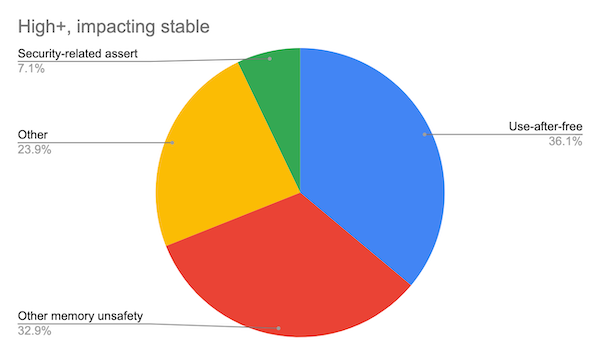
\includegraphics[width=0.7\textwidth]
    {chromium-use-after-free}
  \end{figure}

  \visible<2->{
    Chromium is written in C/C++!\\
    Surely these bugs don't happen in high-level typed languages%
    \alt<3>{ \dots right?}{.}
  }
  
\end{frame}

\begin{frame}[fragile]
  \frametitle{Let's write some OCaml code}

\begin{minted}{OCaml}
let gradeDB : database = Dbm.opendbm "gradeDB" ... in
Dbm.add gradeDB "math" 42;
(* ... *)
Dbm.close gradeDB;
(* ... *)
print_int (Dbm.find gradeDB "literature") (* run-time error! *)
\end{minted}
  
\end{frame}

\begin{frame}[fragile]
  \frametitle{Affe!}

  \begin{onlyenv}<1-3>
\begin{minted}[texcomments=true,escapeinside=\#\#]{OCaml}
let gradeDB : #\tikzcoord{db1}#database#\tikzcoord{db2}# = Dbm.opendbm "gradeDB" ... in
Dbm.add #\tikzcoord{A1}#&!gradeDB#\tikzcoord{A2}# #\tikzcoord{string1}#"math"#\tikzcoord{string2}# 42;
(* ... *)
Dbm.close gradeDB;
(* ... *)
print_int (Dbm.find #\tikzcoord{U1}#&gradeDB#\tikzcoord{U2}# "literature") (* \N compile-time error! *)
\end{minted}
  \end{onlyenv}
  \begin{onlyenv}<4>
\begin{minted}[texcomments=true,escapeinside=\#\#]{OCaml}
let gradeDB #\tikzcoord{eq1}#=#\tikzcoord{eq2}# Dbm.opendbm "gradeDB" ... in
Dbm.add &!gradeDB "math" 42;
(* ... *)
Dbm.close gradeDB;
(* ... *)
print_int (Dbm.find &gradeDB "literature") (* \N compile-time error! *)
\end{minted}
  \end{onlyenv}
  
  \begin{tikzpicture}[remember picture,overlay]
    \begin{onlyenv}<2>
      \node[code,fit=(db1) (db2)] (db) {};
      \node[code,fit=(string1) (string2)] (string) {};
      \node[overlay% ,text width=8.7cm
      ,annot,scale=1.2] at (5,-0.7) {
        Kinds determine usage
        % \begin{itemize}
        % \item Linear (@lin@): Used exactly once $[1]$
        % \item Affine (@aff@): Used at most once $[0-1]$
        % \item Unrestricted (@un@): Used arbitrarily many time $[0-\infty]$
        % \end{itemize}
      };
      \draw[overlay,link] (db) to[out=60,in=-90]
      +(0,1) node[annot,anchor=south]
      {@type database : lin (* Linear kind *)@};
      \draw[overlay,link] (string) to[out=-30,in=180]
      +(1.5,-0.5) node[annot,anchor=west]
      {@type string : un (* Unrestricted kind *)@};
    \end{onlyenv}
    \begin{onlyenv}<3>
      \node[code,fit=(A1) (A2)] (A) {};
      \node[code,fit=(U1) (U2)] (U) {};
      \node[annot,scale=1.2] at ($(A)+(2,-0.8)$) (borrows) {Borrows!};
      \draw[overlay,link,<-] (A) to[out=-30,in=150] (borrows) ;
      \draw[overlay,link,<-] (U) to[out=120,in=-70] (borrows) ;
    \end{onlyenv}
    \begin{onlyenv}<4>
      \node[code,fit=(eq1) (eq2)] (eq) {};
      \draw[overlay,link,<-] (eq) to[out=90,in=-90]
      +(0.5,1) node[annot,scale=1.2,anchor=south]
      {Complete Type Inference};
    \end{onlyenv}
  \end{tikzpicture}
\end{frame}

\begin{frame}{Table of contents}
  \setbeamertemplate{section in toc}[sections numbered]
  \tableofcontents[hideallsubsections]
\end{frame}

\section{Linearity through kinds}


\begin{frame}[fragile]
  \frametitle{Linearity through kinds}
  
  \textbf{Kinds determine usage:}
  \begin{itemize}
  \item Linear (@lin@): Used exactly once $[1]$
  \item Affine (@aff@): Used at most once $[0-1]$
  \item Unrestricted (@un@): Used arbitrarily many time $[0-\infty]$
  \end{itemize}

  \textbf{Examples:}
  \begin{onlyenv}<1>
\begin{minted}[texcomments=true]{OCaml}
type database : lin
type string : un
\end{minted}
  \end{onlyenv}
  \begin{onlyenv}<2>
\begin{minted}[texcomments=true]{OCaml}
type ('a : 'k) list : 'k
\end{minted}
  \end{onlyenv}
  \begin{onlyenv}<3->
\begin{minted}[texcomments=true]{OCaml}
type ('a : 'k) list : 'k
val create_list : ('a : un) => int -> 'a -> 'a list
\end{minted}
    
    \begin{onlyenv}<4>
      We also use \textbf{subkinding}: @un <= aff <= lin@
    \end{onlyenv}
  \end{onlyenv}
\end{frame}


\section{Functions and captures}


\begin{frame}{Table of contents}
  \setbeamertemplate{section in toc}[sections numbered]
  \tableofcontents[hideallsubsections,currentsection]
\end{frame}

\begin{frame}[t,fragile]
  \frametitle{Functions and captures}

\begin{minted}[texcomments=true,escapeinside=\#\#]{OCaml}
let gradeDB = Dbm.open ... 

let #\tikzcoord{fun1}#log_n_close#\tikzcoord{fun2}# msg = 
  printf "Closing: %s" msg;
  Dbm.close #\tikzcoord{db1}#gradeDB#\tikzcoord{db2}#
\end{minted}
  \begin{onlyenv}<3->
    We infer the type:
\begin{minted}[texcomments=true,escapeinside=\#\#]{OCaml}
val log_n_close : string #\tikzcoord{arr1}##$\tarr{\texttt{lin}}$##\tikzcoord{arr2}# unit
\end{minted}
  \end{onlyenv}

  \begin{tikzpicture}[remember picture,overlay]
    \begin{onlyenv}<2->
      \node[code,fit=(fun1) (fun2)] (fun) {};
      \node[code,fit=(db1) (db2)] (db) {};
      \node[annot,scale=1.2]
      at ($(fun)+(5,0.2)$) (capture) {
        Capture!
      };
      \draw[overlay,link] (fun) to[out=20,in=170] (capture) ;
      \draw[overlay,link] (capture) to[out=-90,in=0] (db) ;
    \end{onlyenv}
    \begin{onlyenv}<3->
      \node[code,minimum height=18pt,fit=(arr1) (arr2)] (arr) {};
      \draw[overlay,link,<-] (arr) to[out=-110,in=70]
      +(-1,-1) node[annot,scale=1.2,anchor=north] {
        Usage mode
      };
    \end{onlyenv}
    \begin{onlyenv}<4>
      \node[annot,scale=1.2,red] at ($(arr)+(4,1)$) (warn) {
        \textbf{Warning}: Does not say anything about the arguments!!
      };
      \draw[overlay,link,<-,red] (arr.north) to[out=70,in=-150] (warn.-175) ;
    \end{onlyenv}
  \end{tikzpicture}
\end{frame}

\section{Borrows and regions}

\begin{frame}{Table of contents}
  \setbeamertemplate{section in toc}[sections numbered]
  \tableofcontents[hideallsubsections,currentsection]
\end{frame}

\begin{frame}[t,fragile]{Borrows}
  
  A borrow is a temporary loan of a resource @a@
  \begin{itemize}
  \item
    \textbf{Shared} borrows \tikzcoord{UX1}@&a@\tikzcoord{UX2} are for observing the resource
    % \textbf{Shared} borrows \tikzcoord{UX1}@&a@\tikzcoord{UX2} which are Unrestricted (@un@)
  \item
    \textbf{Exclusive} borrows \tikzcoord{AX1}@&!a@\tikzcoord{AX2} are for modifying the resource
    % \textbf{Exclusive} borrows \tikzcoord{AX1}@&!a@\tikzcoord{AX2} which are Affine (@aff@)
  \end{itemize}

  \begin{onlyenv}<2->
  A correct usage of borrows:
\begin{minted}[texcomments=true,escapeinside=\#\#]{OCaml}
let avg =
  (Dbm.find #\tikzcoord{U1}#&gradeDB#\tikzcoord{U2}# "math" + Dbm.find #\tikzcoord{U3}#&gradeDB#\tikzcoord{U4}# "compsci") / 2
  (* \Y Multiple shared borrows *)
in
Dbm.add #\tikzcoord{A1}#&!gradeDB#\tikzcoord{A2}# "average" avg (* \Y One exclusive borrow *)
\end{minted}
  \end{onlyenv}  
  \begin{tikzpicture}[remember picture,overlay]
    \begin{onlyenv}<2->
      \node[code,color=yellow,fit=(A1) (A2)] (A) {};
      \node[code,color=red,fit=(U1) (U2)] (UA) {};
      \node[code,color=red,fit=(U3) (U4)] (UB) {};
      \node[annot] at ($(UA)+(3,1)$) (un) { Unrestricted -- @un@ } ;
      \draw[link] (un) to[out=180,in=80] (UA) ;
      \draw[link] (un) to[out=0,in=100] (UB) ;
      \node[annot] at ($(A)+(2,-1)$) (aff) { Affine -- @aff@ } ;
      \draw[link] (aff) to[out=180,in=-80] (A) ;
    \end{onlyenv}
    \node[code,color=yellow,fit=(AX1) (AX2)] {};
    \node[code,color=red,fit=(UX1) (UX2)] {};
  \end{tikzpicture}
\end{frame}


\begin{frame}[fragile]
  \frametitle{Borrows -- Example of uses}

% \begin{onlyenv}<2>
% \begin{minted}[texcomments=true]{OCaml}
% let gradeDB = ... in
% let avg =
%  let grade topic = Dbm.find &gradeDB topic in (* \Y Capture *)
%  (grade "math" + grade "compsci") / 2
% in
% Dbm.add &!gradeDB "average" avg (* \Y Exclusive borrow *)
% \end{minted}
% \end{onlyenv}
\begin{onlyenv}<1>
  \textbf{Rule 1}: Cannot use a borrow and the resource itself simultaneously
\begin{minted}[texcomments=true]{OCaml}
let gradeDB = ... in
f (gradeDB, &gradeDB) (* \N Conflicting use and borrow! *)
\end{minted}
\end{onlyenv}%
\begin{onlyenv}<2>
  \textbf{Rule 2}: Cannot use an exclusive borrow and any other borrow simultaneously
\begin{minted}[texcomments=true]{OCaml}
let gradeDB = ... in
f (&!gradeDB, &gradeDB) (* \N Conflicting borrows! *)
\end{minted}
\end{onlyenv}%
\begin{onlyenv}<3->
  \textbf{Rule 3}: Borrows must not escape
  \begin{onlyenv}<3>
\begin{minted}[texcomments=true,escapeinside=\#\#]{OCaml}
let f () = 
  let gradeDB = ... in
  #\tikzcoord{R1}#let x = (&gradeDb, "mygrades") in#\tikzcoord{R2}#
  #\tikzcoord{R3}#x#\tikzcoord{R4}#
  (* \N Borrow escaping its scope! *)
\end{minted}
  \end{onlyenv}
  \begin{onlyenv}<4->
\begin{minted}[texcomments=true,escapeinside=\#\#]{OCaml}
let f () = 
  let gradeDB = ... in
  #\tikzcoord{R1}#{| let x = (#\tikzcoord{B1}#&gradeDb#\tikzcoord{B2}#, "mygrades") in#\tikzcoord{R2}#
  #\tikzcoord{R3}#x |}#\tikzcoord{R4}#
  (* \N Borrow escaping its scope! *)
\end{minted}
  \end{onlyenv}%
  \begin{tikzpicture}[remember picture,overlay]%
    \begin{onlyenv}<4->
      \node[code,rounded corners=0,color=red,fit=(R1) (R2)] {};
      \node[code,rounded corners=0,minimum height=15pt,yshift=1pt,color=red,fit=(R3) (R4)] {};
      \node[code,opacity=0,fit=(B1) (B2)] (B) {};
    \end{onlyenv}
    \begin{onlyenv}<5->
      \draw[link,<-] (B.10) to[in=180,out=40] ++(0.5,0.5) node[annot, anchor=west] {
        @&gradeDb : &(database, un_2)@
      };
      \draw[link,<-] (R2) to[in=90,out=-10] ++(1.5,-0.5) node[annot, anchor=north] {
        Region nesting level: 1
      };
    \end{onlyenv}
  \end{tikzpicture}%
  \visible<5>{%
    \textbf{Indexed} kinds ensure that borrows do not escape!

    Borrows of index $2$ cannot escape a region of index $1$.
  }
\end{onlyenv}%
\end{frame}

% \begin{frame}[fragile]{API}

%   {\Large The \texttt{Dbm} API:}
% \begin{minted}[texcomments=true]{OCaml}
% type database : lin
% val find : &(database,'k) -> string -{'k}> int
% val add : &!(database,'k) -> string -{'k}> int -{'k}> unit
% \end{minted}
  
% \end{frame}
  
  % \begin{tikzpicture}[remember picture,overlay]
  %   \begin{onlyenv}<2->
  %     \node[code,color=yellow,fit=(A1) (A2)] {};
  %     \node[code,color=red,fit=(U1) (U2)] {};
  %     \node[code,color=red,fit=(U3) (U4)] {};
  %   \end{onlyenv}
  %   \node[code,color=yellow,fit=(AX1) (AX2)] {};
  %   \node[code,color=red,fit=(UX1) (UX2)] {};
  % \end{tikzpicture}

\begin{frame}[fragile]
  \frametitle{Everything together}

  The @Database@ API:
\begin{minted}[texcomments=true,escapeinside=\#\#]{OCaml}
type database : lin
val find : &(database,'k) -> string #$\tarr{\texttt{'k}}$# int
val add : &!(database,'k) -> string #$\tarr{\texttt{'k}}$# int #$\tarr{\texttt{'k}}$# unit
\end{minted}
  
  \begin{onlyenv}<2->
    A simple use:
  \end{onlyenv}
  \begin{onlyenv}<2>
\begin{minted}[texcomments=true]{OCaml}
let gradeDB = ... in
let avg =
  (Dbm.find &gradeDB "math" + Dbm.find &gradeDB "compsci") / 2

in
Dbm.add &!gradeDB "average" avg
\end{minted}
  \end{onlyenv}
  \begin{onlyenv}<3>
\begin{minted}[texcomments=true]{OCaml}
let gradeDB = ... in
let avg =
  let grade subject = Dbm.find &gradeDB subject in (* \Y Capture *)
  (grade "math" + grade "compsci") / 2
in
Dbm.add &!gradeDB "average" avg
\end{minted}
  \end{onlyenv}
  \begin{onlyenv}<4>
\begin{minted}[texcomments=true]{OCaml}
let gradeDB = ... in
let avg =
  let grade = Dbm.find &gradeDB in (* \Y Partial application *)
  (grade "math" + grade "compsci") / 2
in
Dbm.add &!gradeDB "average" avg
\end{minted}
  \end{onlyenv}
  \begin{onlyenv}<5->
    \begin{onlyenv}<5>%
\begin{minted}[texcomments=true]{OCaml}
let average db subjects = 
  List.map (Dbm.find db) subjects / List.length subjects
let main () =
  let gradeDB = ... in
  let avg = average &gradeDB ["math";"compsci";...] in
  Dbm.add &!gradeDB "average" avg
\end{minted}
    \end{onlyenv}%
    \begin{onlyenv}<6>%
\begin{minted}[texcomments=true,escapeinside=\#\#]{OCaml}
let average db subjects #\tikzcoord{eq1}#=#\tikzcoord{eq2}#
  List.map (Dbm.find db) subjects / List.length subjects
let main () =
  let gradeDB = ... in
  let avg = #\tikzcoord{R1}#{| average &gradeDB ["math";"compsci";...] |}#\tikzcoord{R2}# in
  #\tikzcoord{R3}#{| Dbm.add &!gradeDB "average" avg |}#\tikzcoord{R4}#
\end{minted}
    \end{onlyenv}%
  \end{onlyenv}%
  \begin{tikzpicture}[remember picture,overlay]%
    \begin{onlyenv}<6>
      \node[code,fit=(eq1) (eq2)] (eq) {};
      \draw[overlay,link,<-] (eq) to[out=60,in=180]
      +(0.5,0.5) node[annot,scale=1.2,anchor=west]
      {No type annotation};
      \node[code,rounded corners=0,color=red,fit=(R1) (R2)] (RA) {};
      \node[code,rounded corners=0,color=yellow,fit=(R3) (R4)] (RB) {};
      \node[annot,scale=1.2] at ($(R4)+(1,-1)$) (AR) {Disjoint regions};
      \draw[link] (AR) to[out=90,in=-40] (RA.-8);
      \draw[link] (AR) to[out=180,in=-40] (RB.-8);
    \end{onlyenv}
  \end{tikzpicture}%
\end{frame}

\section{Inference and constraints}

\begin{frame}{Table of contents}
  \setbeamertemplate{section in toc}[sections numbered]
  \tableofcontents[hideallsubsections,currentsection]
\end{frame}

% \begin{frame}{Inference and constraints}

%   \begin{enumerate}
%   \item Elaborate regions
%   \item Generate constraints for type, linearity and escape checks
%   \item Solve the constraints
%   \item Simplify the resulting types
%   \end{enumerate}
% \end{frame}

% \begin{frame}[fragile]
%   \frametitle{Inference in action}
%   \begin{onlyenv}<1>%
% \begin{minted}[texcomments=true]{OCaml}
% let average db subjects = 
%   List.map (Dbm.find db) subjects / List.length subjects

% let main () =
%   let gradeDB = ... in
%   let avg = average &gradeDB ["math";"compsci";...] in
%   Dbm.add &!gradeDB "average" avg
% \end{minted}
%   \end{onlyenv}%
%   \begin{onlyenv}<2>%
% \begin{minted}[texcomments=true,escapeinside=\#\#]{OCaml}
% let average db subjects =
%   List.map (Dbm.find db) subjects / List.length subjects

% let main () =
%   let gradeDB = ... in
%   let avg = #\tikzcoord{R1}#{| average &gradeDB ["math";"compsci";...] |}#\tikzcoord{R2}# in
%   #\tikzcoord{R3}#{| Dbm.add &!gradeDB "average" avg |}#\tikzcoord{R4}#
% \end{minted}
%   \end{onlyenv}%
%   \begin{tikzpicture}[remember picture,overlay]%
%     \begin{onlyenv}<2>
%       \node[code,rounded corners=0,color=red,fit=(R1) (R2)] (RA) {};
%       \node[code,rounded corners=0,color=yellow,fit=(R3) (R4)] (RB) {};
%     \end{onlyenv}
%   \end{tikzpicture}%
% \end{frame}

\begin{frame}[fragile,t,shrink]
  \frametitle{Inference in action}
  \begin{center}
    \begin{tikzpicture}[xscale=1,yscale=0.8]
      \node[annot,text width=11.5cm,scale=0.5] at (0,4) (S1) {%
\begin{minted}[texcomments=true]{OCaml}
let average db subjects = 
  List.map (Dbm.find db) subjects / List.length subjects

let main () =
  let gradeDB = ... in
  let avg = average &gradeDB ["math";"compsci";...] in
  Dbm.add &!gradeDB "average" avg
\end{minted}
      };
      
      \node[annot,text width=12cm,scale=0.5] at (8,4) (S2) {%
\begin{minted}[texcomments=true,escapeinside=\#\#]{OCaml}
let average db subjects =
  List.map (Dbm.find db) subjects / List.length subjects

let main () =
  let gradeDB = ... in
  let avg = #\tikzcoord{R1}#{| average &gradeDB ["math";"compsci";...] |}#\tikzcoord{R2}# in
  #\tikzcoord{R3}#{| Dbm.add &!gradeDB "average" avg |}#\tikzcoord{R4}#
\end{minted}
        \tikz[remember picture,overlay]{
          \node[code,rounded corners=0,color=red,fit=(R1) (R2)] (RA) {};
          \node[code,rounded corners=0,color=yellow,fit=(R3) (R4)] (RB) {};
        }%
      };

      \draw[link,->] (S1) to node[midway,above,sloped] {1. Elaborate} (S2) ;
      \draw[link,->] (S1) to node[midway,below,sloped] {regions} (S2) ;
      
      \visible<2->{
        \node[annot,text width=4.8cm] at (8,0) (S3) {%
          \vspace{-1em}
          \begin{align*}
            \E = &(\tvar_f : \kvar_f)
                 (\tvar_x : \kvar_x)\dots\\
            C = &(\tvar_f \leq \gamma \tarr{\kvar_1} \beta )
                \Cand
                (\gamma \leq \tvar_x)\\
                &\Cand
                (\beta \times  \tvar_x \leq \alpha_r)
                \Cand
                  (\kvar_x \leq \kun)\\
                 &\Cand \dots
          \end{align*}
        };
        \draw[link,->] (S2) to
        node[midway,right,text width=3cm] {2. Generate\\ constraints}
        (S3);
      }

      \begin{onlyenv}<3->
        \node[annot,text width=10.5cm,scale=0.7] at (0.7,1) (S4) {
          @val average : 'k_2 . &(database,'k) -{'k_2}> string list -{'k}> int list@
        };
        \draw[link,->] ($(S3.west)+(0,1)$) to
        node[midway, above, sloped] {3. Solve}
        node[midway, below, sloped] {constraints}
        (S4.east);
      \end{onlyenv}
      
      \begin{onlyenv}<4->
        \node[annot,text width=9.7cm,scale=0.7] at (0.7,-1) (S5) {
          @val average : &(database,'k) -> string list -{'k}> int list@
        };
        \draw[link,->] (S4) to
        node[midway, left] {4. Simplify}
        node[midway, right] {types}
        (S5);
      \end{onlyenv}

    \end{tikzpicture}
  \end{center}

  \only<1>{%
    1. Infer the placement of region based on the position of borrows and the borrowing rules.
  }%
  \only<2>{%
    2. Generate custom constraints based on HM(X).
  }%
  \only<3>{%
    3. Solve the constraints using a custom algorithm and obtain principal type schemes.
  }%
  \only<4>{%
    4. Simplify the obtained type scheme by leveraging subkinding
  }%

\end{frame}
\section*{Conclusion}



\begin{frame}
  \frametitle{The \lang language -- Summary}

  Prototype: \url{https://affe.netlify.com/}  
  
  \begin{itemize}
  \item[\Y] Linearity, Closures, Borrows and Regions\\
    $\Rightarrow$ Good support for both imperative and functional programming
  \item[\Y] Support managed and unmanaged objects
  \item[\Y] Principal type inference
  \item[\N] No flow sensitivity
  \item[\N] No concurrency story (yet)
  \end{itemize}
  
  Many examples in the paper: files, session types, semi-persistent arrays, iterators, connection pools, \dots
\end{frame}

\begin{frame}
  \frametitle{The theory -- Summary}

  \begin{itemize}
  \item A Syntax-directed type system for \lang\\
    $\Rightarrow$ How to encode borrows into an ML-style type-system
  \item A formal semantics that takes allocations into account (+ proof of soundness)
  \item An inference algorithm for \lang:
    \begin{itemize}
    \item An extension of HM(X) with kinds
    \item A novel constraint systems to encode linearity and borrows
    \item A constraint solving algorithm, and its proof of completeness
    \end{itemize}
  \end{itemize}
\end{frame}

\begin{frame}[standout]

  \centering\Huge\texttt{Close(Talk)}
  
\end{frame}

\bibliography{biblio}

\end{document}

%%% Local Variables:
%%% mode: latex
%%% TeX-command-extra-options: "-shell-escape"
%%% TeX-master: "slides-icfp"
%%% End:
